\section{Model selection}

We tried severall models: linear regression, K-nearest neightbors (KNN), multi-layer perceptron and a random forest. For each model except the linear regression, we choosed to tweak severall well chosen hyperparameters and used a searching algorithm along with cross-validation (5 folds) to find the best hyperparameters for each model. A common searching algorithm is \textbf{Grid Search} that will test every possible combination of hyperparameters. However, it can be computationaly intensive if the search space is wide which is often the case since we don't want to miss the optimal parameters. Another approach is to use \textbf{Random Search}. With this approach, we can also draw hyperparameter configurations from distributions besides discrete sets and the random search will randomly select a combination of hyperparameters among the ones defined instead of doing an exhaustive search. It allows to explore a wide range of hyperparameter configurations with time-efficiency. Looking at the result of the random search, we can identify the area where the results are promising, tighten our ranges and perform a random search again. Although this algorithm being less computationaly intensive, it can be time consuming of running and running again the random search to find the best set of hyperparameters. 

\begin{figure}[H]
	\centering
	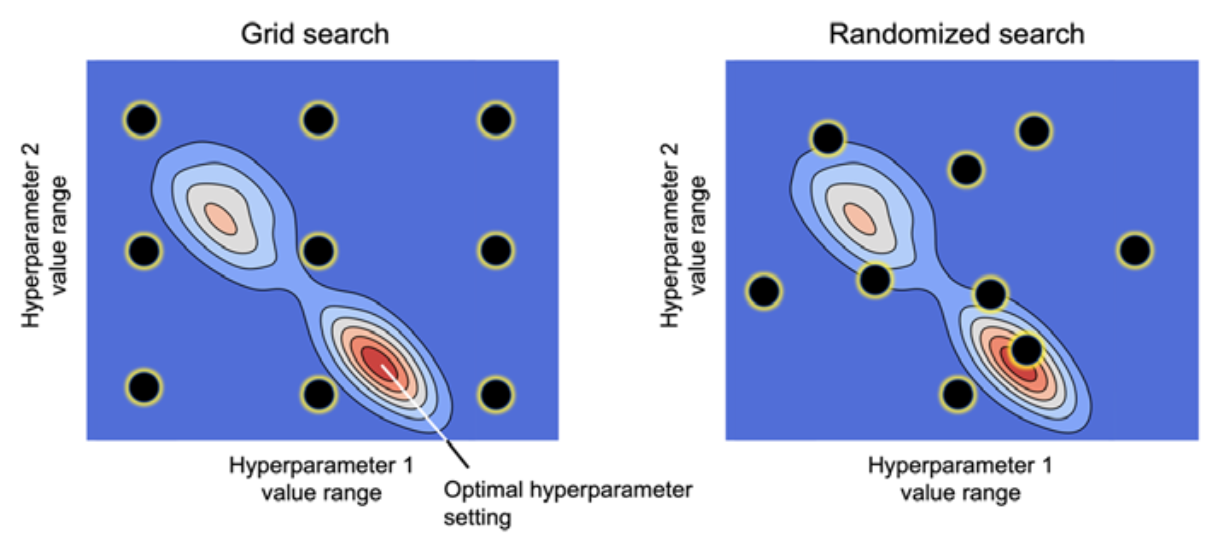
\includegraphics{figures/grid_search_vs_random_search.png}
	\caption{Comparison of grid search and randomized for sampling $9$ different hyperparameter configurations}
	\label{fig:gridsearch_vs_randomsearch}
\end{figure}

A third approach and the one we tried in this project is to perform a \textbf{Bayesian Search} which is basically similar to random search but modelise the hyperparameters space probabilisticly to optimize the research of the best set of hyperparameters. For each model, we run a 5-fold cross-validation to avoid overfitting and we compute the validation score as well as the test score that's been computed on a part of the $X_1$ dataset that has not been used to train any of our models.

\subsection{Linear regression}

The linear regression has no hyperparameters to tune so we just ran a cross-validation for each set of features we decided to keep. The results show us that ... 

\begin{table}[H]
	\centering
	\begin{tabular}{ccc} \toprule
	  & \multicolumn {2}{c}{scores} \\\cmidrule(lr) {2-3}
	  \#features         & validation rmse (\$)             & test rmse (\$) \\\hline
	  $5$        		& $7.986e07$                      	& $8.618e07$ \\
	  $10$        		& $8.874e07$                        & $8.905e07$ \\
	  $15$        		& $8.491e07$                        & $8.764e07$ \\
	  $20$             	& $7.134e07$                        & $7.875e07$ \\
	  $30$             	& $6.980e07$                        & $7.701e07$ \\
	  \\\hline
	\end{tabular}
	\caption{Cross-validation results of linear regression model}
	\label{tab:linear-regression-results}
\end{table}

\subsection{K-Nearest Neighbors}

For the K-Nearest Neighbors model, we need to take care of adjusting the number of neighbors hyperparameter. Indeed, a value too low will induce overfitting and a value too high will induce underfitting. We ran a bayesian search with $12$ iterations.

\begin{table}[H]
	\centering
	\begin{tabular}{ccc} \toprule
	  & \multicolumn {2}{c}{scores} \\\cmidrule(lr) {2-3}
	  \#features         & validation rmse (\$)             & test rmse (\$) \\\hline
	  $5$        		& $6.357e07$                      	& $7.738e07$ \\
	  $10$        		& $6.236e07$                        & $7.404e07$ \\
	  $15$        		& $6.172e07$                        & $7.455e07$ \\
	  $20$             	& $6.341e07$                        & $7.281e07$ \\
	  $30$             	& $6.386e07$                        & $7.226e07$ \\
	  \\\hline
	\end{tabular}
	\caption{Cross-validation results of K-Nearest Neighbors model}
	\label{tab:knn-results}
\end{table}

\subsection{Multi-Layer Perceptron}

\begin{table}[H]
	\centering
	\begin{tabular}{ccc} \toprule
	  & \multicolumn {2}{c}{scores} \\\cmidrule(lr) {2-3}
	  \#features         & validation rmse (\$)             & test rmse (\$) \\\hline
	  $5$        		& $6.267e07	$                      	& $8.023e07$ \\
	  $10$        		& $6.255e07$                        & $7.973e07$ \\
	  $15$        		& $6.355e07$                        & $7.793e07$ \\
	  $20$             	& $6.156e07$                        & $8.117e07$ \\
	  $30$             	& $6.339e07$                        & $7.930e07$ \\
	  \\\hline
	\end{tabular}
	\caption{Cross-validation results of Multi-Layer perceptron model}
	\label{tab:mlp-results}
\end{table}

\subsection{Random Forest}

A random forest is an ensemble technique that combines multiple decision trees. As a consequence, it has a better generalization performance than a single decision tree due to randomness which decrease the model's variance. Another thing to note is that it is little sensitive to outliers and do not require much hyperparameters tuning.

\begin{table}[H]
	\centering
	\begin{tabular}{ccc} \toprule
	  & \multicolumn {2}{c}{scores} \\\cmidrule(lr) {2-3}
	  \#features         & validation rmse (\$)             & test rmse (\$) \\\hline
	  $5$        		& $6.267e07	$                      	& $8.023e07$ \\
	  $10$        		& $6.255e07$                        & $7.973e07$ \\
	  $15$        		& $6.355e07$                        & $7.793e07$ \\
	  $20$             	& $6.156e07$                        & $8.117e07$ \\
	  $30$             	& $6.339e07$                        & $7.930e07$ \\
	  \\\hline
	\end{tabular}
	\caption{Cross-validation results of Random Forest model}
	\label{tab:rf-results}
\end{table}